\chapter{Introduction}
Automatic 3D reconstruction of real objects plays an important role in many applications such as animation, virtual reality, and gaming. A widely used approach to reconstruct an object is by using a 3D laser range scanner. Since range scanners have limited field of view, acquisition of 3D geometry of an object requires taking several scans from different viewpoints. The main difficulty with this method is to combine these scans into a unique surface representing the object. This typically involves two steps. First, all the scans must be transformed into the same coordinate system by a process known as surface registration. Second, the registered scans must be integrated into a single model by a process known as surface integration. In this paper we focus on surface integration, assuming the scans have been acquired and registered in a common coordinate system.

\section{First section}
Existing surface integration methods for range images can be classified into two categories: volume-based and mesh-based. Volume-based methods \cite{Claes:VolM05,Curless:VolM96,Masuda:VolM02,Hoppe:VolM97,Sato:VolM97,Sun:VolM03} convert range images into an intermediate volumetric representation using a signed distance function and extract the final surface using a polygonizing algorithm. These methods can handle objects of arbitrary topology and are considered to be robust with respect to scanning noise, outliers and registration errors. The choice of appropriate voxel size is important for these methods \cite{Claes:VolM05,Curless:VolM96}. If the voxel size is too large, then features smaller than the voxel size are missed and opposite surfaces of a narrow region will be merged. If the voxel size is too small, then in the presence of scanning noise or registration errors, corresponding surfaces will be reconstructed as separate surfaces. It still remains unanswered as to what extent the signed distance function computed on the discretized space is sensitive to the presence of noisy data. It is also not clear how to choose an appropriate voxel size when the input range images have both small features and registration errors. \\

Mesh-based methods \cite{Pito:MeshM96,Rutishauser:MeshM94,Sappa:MeshM00,Soucy:MeshM92,Soucy:MeshM95,Sun:MeshM00,Turk:MeshM94,Zhou:MeshM06} directly integrate range images into a single mesh. These methods do not need an intermediate representation. Hence, they are faster and require less memory compared to volumetric methods. In addition, they are more amenable to data reduction during processing which makes them more feasible for use with very large meshes. Existing methods are, however, sensitive to scanning errors and do not work well on objects with large surface curvature \cite{Curless:VolM96}.

\begin{figure}[t]
    \centering
    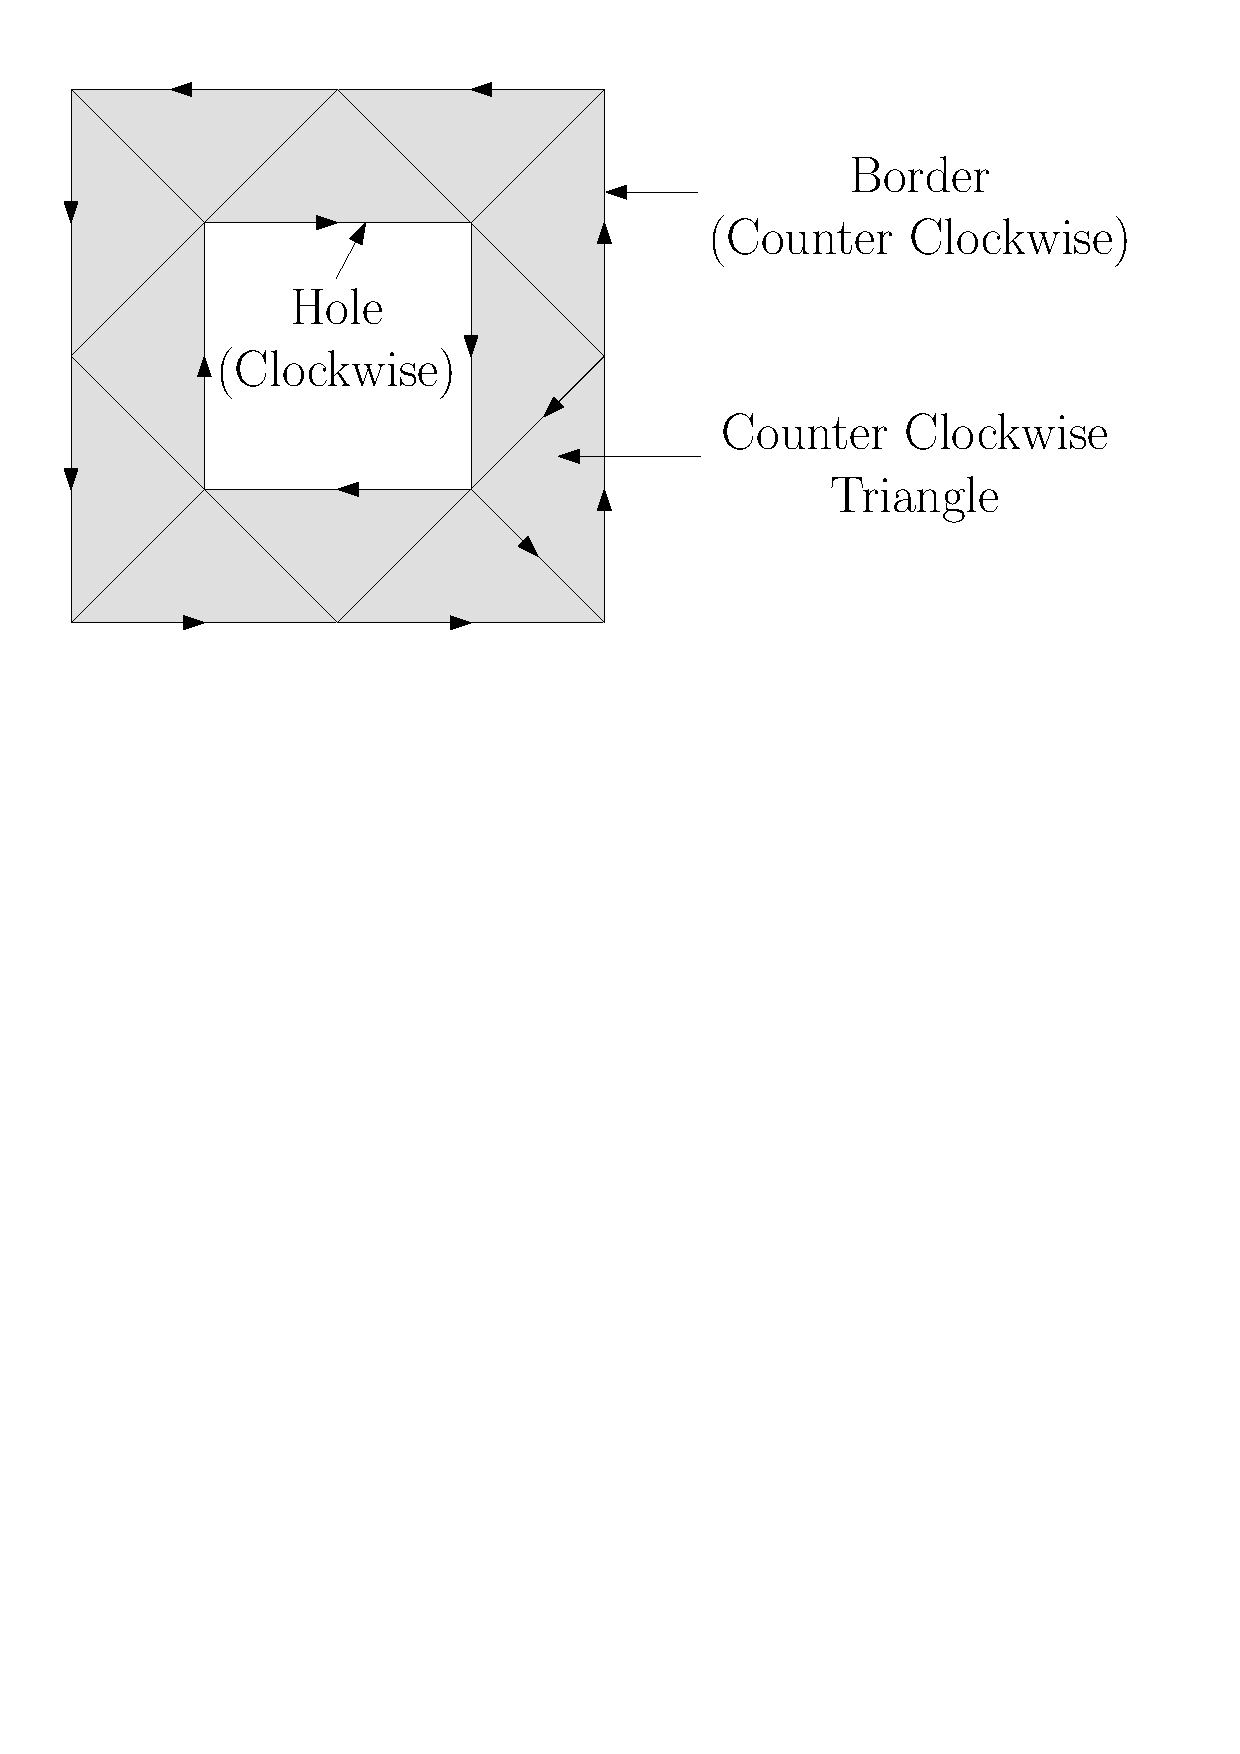
\includegraphics[width=5in]{border}
    \caption[Boundary edges]{Boundary edges.}
    \label{fig:Ch1-border}
\end{figure}
% \subsection{Row dispatcher}

% \begin{macro}{\cals@row@dispatch}
% Depending if the current row has a rowspan cell or not,
% the execution is different.
%    \begin{macrocode}
\newcommand\cals@row@dispatch{%
\ifx b\cals@current@context
 \cals@ifInRspan\iftrue
  \cals@row@dispatch@span
 \else
  \cals@row@dispatch@nospan
 \fi
\else
 \cals@row@dispatch@nospan
\fi}
%    \end{macrocode}
% \end{macro}

% \begin{macro}{\cals@row@dispatch@nospan}
% After a row is typeset in a box, this macro decides what to do next.
% Usually, it should just add decorations and output the row.
% But if a table break is required, it should put the current row
% to backup, typeset the footer, the break, the header and only then 
% the row from the backup. Summary of main parameters:
% \begin{itemize}
% \item rowsep from the last row (|\cals@last@rs|) and the
%   last context (|\cals@last@context|)
% \item current row (|\cals@current@row|), its decorations
%  (|\cals@current@cs|, |\cals@current@rs@above|,
%  |\cals@current@rs@below|) and context (|\cals@current@context|)
% \end{itemize}
%    \begin{macrocode}
\newcommand\cals@row@dispatch@nospan{%
%    \end{macrocode}
% The header and footer rows are always typeset without further
% considerations.
%    \begin{macrocode}
\let\cals@last@context@bak=\cals@last@context
\ifx h\cals@current@context \else
\ifx f\cals@current@context \else
%    \end{macrocode}
% In the body, if a break is required: do it.
%    \begin{macrocode}
\cals@ifbreak\iftrue
 \setbox\cals@backup@row=\box\cals@current@row
 \setbox\cals@backup@cs=\box\cals@current@cs
 \let\cals@backup@rs@above=\cals@current@rs@above
 \let\cals@backup@rs@below=\cals@current@rs@below
 \let\cals@backup@context=\cals@current@context
 \cals@tfoot@tokens
 \lastrule
 \cals@issue@break
 \cals@thead@tokens
 \setbox\cals@current@row=\box\cals@backup@row
 \setbox\cals@current@cs=\box\cals@backup@cs
 \let\cals@current@rs@above=\cals@backup@rs@above
 \let\cals@current@rs@below=\cals@backup@rs@below
 \let\cals@current@context=\cals@backup@context
\fi\fi\fi
%    \end{macrocode}
% Typeset the row. If the width of the row is more than hsize, then
% the issue-code should not fit the row to hsize.
%    \begin{macrocode}
\ifdim\wd\cals@current@row>\hsize\relax
\def\cals@tohsize{}%
\fi
\cals@issue@row
%    \end{macrocode}
% Consider a table such that thead+row1 do not fit to a page
% (see the unit test |regression/test_010_wrongbreak|).
% Without the next code, the following happens:
% thead and row1 are typeset, but the output procedure is not
% executed yet. Therefore, when row2 is ready, we detect that
% a table break is required and create it. Then the output procedure
% moves thead+row1 on the next page. The result:
% thead and row1 on one page, row2 and the rest on the next page
% instead of the whole table on one page.
% Solution: force a run of the output procedure after
% the first row of a table chunk.
%    \begin{macrocode}
\ifx b\cals@last@context
  {\dimen0=\pagetotal\relax
  \advance\dimen0 by \cals@tfoot@height\relax
  \advance\dimen0 by -\pagegoal
  \ifdim\dimen0>0pt\relax
    \vskip\dimen0
    \penalty9999 % with 10000, the output page builder is not called
    \vskip-\dimen0\relax
  \fi
  }%
\fi
}
%    \end{macrocode}
% \end{macro}

% \begin{macro}{\cals@row@dispatch@span}
% The only specific thing to rowspanned rows is that we should not
% allow breaks between the rows in one group. We put these rows
% to one box, and process this big box as a big row.
%    \begin{macrocode}
\newcommand\cals@row@dispatch@span{%
%    \end{macrocode}
% Output the row to the backup box. If the row is the first
% row in the span, let its decorations will be the decorations
% for the future big row. Also, reset the values of leftskip
% and rightskip to avoid adding them twice, once in a individual
% row, and once to the common span box.
%    \begin{macrocode}
\ifvoid\cals@backup@row
 \setbox\cals@backup@row=\vbox{\box\cals@current@row}%
 \setbox\cals@backup@cs=\box\cals@current@cs
 \let\cals@backup@rs@above=\cals@current@rs@above
 \let\cals@backup@last@rs@below=\cals@last@rs@below
 \let\cals@backup@context=\cals@last@context
 \cals@backup@leftskip=\leftskip\relax
 \cals@backup@rightskip=\rightskip\relax
 \let\cals@backup@tohsize=\cals@tohsize
 \leftskip=0pt\relax \rightskip=0pt\relax \def\cals@tohsize{}%
\else
 \setbox\cals@backup@row=\vbox{\unvbox\cals@backup@row
  \cals@issue@row}%
\fi
\let\cals@last@rs@below=\cals@current@rs@below
\let\cals@last@context=\cals@current@context
%    \end{macrocode}
% If this is the last row of the span, create the fake big row
% and use the normal dispatcher.
%
%    \begin{macrocode}
\cals@ifLastRspanRow\iftrue
 \setbox\cals@current@row=\box\cals@backup@row
 \setbox\cals@current@cs=\box\cals@backup@cs
 \let\cals@current@rs@above=\cals@backup@rs@above
 \let\cals@last@rs@below=\cals@backup@last@rs@below
 \let\cals@last@context=\cals@backup@context
 \leftskip=\cals@backup@leftskip
 \rightskip=\cals@backup@rightskip
 \let\cals@tohsize=\cals@backup@tohsize
 \cals@row@dispatch@nospan
\fi
}
%    \end{macrocode}
% \end{macro}

% \begin{macro}{\cals@backup@row}
% \begin{macro}{\cals@backup@cs}
% Boxes and skips for backup.
%    \begin{macrocode}
\newbox\cals@backup@row
\newbox\cals@backup@cs
\newskip\cals@backup@leftskip
\newskip\cals@backup@rightskip
%    \end{macrocode}
% \end{macro}
% \end{macro}

% To decide on table breaks and row separation decorations,
% we need to trace context.

% \begin{macro}{\cals@current@context}
% The context of the current row. Possible values,
% set as a "|\let|" to a character:
% \begin{itemize}
% \item n: no context, should not happen when the value is required
% \item h: table header
% \item f: table footer
% \item b: table body
% \end{itemize}
% \end{macro}

% \begin{macro}{\cals@last@context}
% The context of the previous row. Possible values, set as a
% "|\let|" to a character:
% \begin{itemize}
% \item n: there is no previous row (not only the start of a table,
%   but also the start of a table chunk)
% \item h, f, b: table header, footer, body
% \item r: a last rule of the table (or its chunk) is just output.
%   This status is used to allow multiple calls to |\lastrule|.
%   Probably the use of |current| instead of |last| is more logical,
%   but using |last| is more safe. Who knows if an user decides to use
%   |\lastrule| somewhere in a middle of a table.
% \end{itemize}
% \end{macro}

% \begin{macro}{\cals@ifbreak}
% Table breaks can be manual or automatic. The first is easy,
% the second is near to impossible if we take into account
% table headers and footer. The following heuristic seems good.
% 
% Check if the current row plus the footer fits to the
% rest of the page. If not, a break is required. This approach
% is based on two assumptions:
% \begin{itemize}
% \item the height of the footer is always the same, and
% \item any body row is larger than the footer.
% \end{itemize}
%
% More precise and technical description: |\cals@ifbreak| decides
% if an automatic table break is required and leaves the
% macro |\cals@iftrue| (yes) or |\cals@iffalse| (no) in the input stream.
% If the user sets |\cals@tbreak@tokens| (using |\tbreak|),
% break is forced. Otherwise, no break is allowed:
% \begin{itemize}
% \item inside a box (= inside a float)
% \item In the header
% \item In the footer
% \item Immediately after the header
% \item At the beginning of a chunk of a table.
% \end{itemize}
% Otherwise break is recommended when
% the sum of the height of the current row and of the footer part
% is greater as the rest height of the page.
% The implicit first parameter is used for if-fi balancing,
% see |\cals@iftrue|.
%    \begin{macrocode}
\newcommand\cals@ifbreak[1]{}
\def\cals@ifbreak{%
\let\cals@tmp=\cals@iffalse
\let\cals@tmpII=\cals@iftrue
\ifx\relax\cals@tbreak@tokens
 \ifinner\else
  \ifx h\cals@current@context \else
   \ifx f\cals@current@context \else
    \ifx h\cals@last@context \else
     \ifx n\cals@last@context \else
       \dimen0=\pagetotal\relax
       \advance\dimen0 by \ht\cals@current@row\relax
       %\showthe\ht\cals@current@row\relax
       \ifx \cals@tfoot@tokens\relax \else
         %\show\cals@tfoot@height\relax
         \advance\dimen0 by \cals@tfoot@height\relax
       \fi
       %\showthe\dimen0\relax
       \ifdim \dimen0>\pagegoal\relax
         \let\cals@tmp=\cals@tmpII
       \fi
 \fi\fi\fi\fi\fi
\else \let\cals@tmp=\cals@tmpII % tbreak@tokens
\fi
\cals@tmp}
%    \end{macrocode}
% \end{macro}

% \begin{macro}{\cals@issue@break}
% By default, force a page break, otherwise use user's tokens
% set by |\tbreak|.
%    \begin{macrocode}
\newcommand\cals@issue@break{\ifx \relax\cals@tbreak@tokens \penalty-10000 %
\else \cals@tbreak@tokens \fi
\let\cals@tbreak@tokens=\relax
\let\cals@last@context=n}
%    \end{macrocode}
% \end{macro}

% \begin{macro}{\cals@set@tohsize}
% \begin{macro}{\cals@tohsize}
% Table row contains not only the row itself, but also |\leftskip|
% and |\rightskip|. Now the dilemma. If the row is just |\hbox|,
% than the glue component is ignored, and the table always aligned
% left. On the other side, if the row is |\hbox to \hsize|, then
% the user gets underfulled boxes. A simple solution is to
% switch on and off the |hsize|-part depending on the skips.
%    \begin{macrocode}
\newcommand\cals@tohsize{}
\newcommand\cals@set@tohsize{\def\cals@tohsize{}%
\ifnum\gluestretchorder\leftskip>0\relax \def\cals@tohsize{to \hsize}\fi
\ifnum\gluestretchorder\rightskip>0\relax \def\cals@tohsize{to \hsize}\fi
}
%    \end{macrocode}
% \end{macro}
% \end{macro}

% \begin{macro}{\cals@activate@rtl}
% \begin{macro}{\cals@deactivate@rtl}
% \begin{macro}{\cals@hbox}
% For bidi support, use |\hboxR| instead of |\hbox|.
% Actually, more is required for bidi support, and
% these macros are retained only as "legacy".
% Otherwise I'd move the code into the beginning of `calstable`.
%    \begin{macrocode}
\newcommand\cals@hbox{}
\newcommand\cals@activate@rtl{\let\cals@hbox=\hboxR}
\newcommand\cals@deactivate@rtl{\let\cals@hbox=\hbox}
\cals@deactivate@rtl
%    \end{macrocode}
% \end{macro}
% \end{macro}
% \end{macro}

% \begin{macro}{\cals@issue@rowsep@alone}
% Typesets the top (or bottom) frame of a table:
% combines |\cals@current@rs@above| and |\cals@framers@width|
% and outputs the row separator.
%    \begin{macrocode}
\newcommand\cals@issue@rowsep@alone{%
\setbox0=\cals@hbox\cals@tohsize{%
 \cals@hskip@lr\leftskip\rightskip
 \cals@rs@sofar@reset
 \cals@rs@joinOne\cals@framers@width\cals@current@rs@above
 \cals@rs@sofar@end
 \cals@hskip@lr\rightskip\leftskip}%
\ht0=0pt \dp0=0pt \box0 }
%    \end{macrocode}
% \end{macro}

% \begin{macro}{\cals@issue@rowsep}
% Combine row separations |\cals@last@rs@below| and |\cals@current@rs@above|,
% taking into considiration the width of the rule:
% \begin{itemize}
% \item n to h, f, b (the top frame): use |\cals@framers@width|
%   and ignore |last@rs@below| because we don't have it
% \item h to h, b to b, f to f (the usual separator): use |\cals@rs@width|
% \item for all other combinations (header to body, body to footer),
% including impossible: use |\cals@bodyrs@width|
% \end{itemize}
%    \begin{macrocode}
\newcommand\cals@issue@rowsep{%
\ifx n\cals@last@context \cals@issue@rowsep@alone \else
 \ifx \cals@last@context\cals@current@context
   \let\cals@tmpIII=\cals@rs@width     \else
   \let\cals@tmpIII=\cals@bodyrs@width \fi
 \setbox0=\cals@hbox\cals@tohsize{%
  \cals@hskip@lr\leftskip\rightskip
  \cals@rs@sofar@reset
  \cals@rs@joinTwo\cals@tmpIII\cals@last@rs@below\cals@current@rs@above
  \cals@rs@sofar@end
  \cals@hskip@lr\rightskip\leftskip}%
 \ht0=0pt \dp0=0pt \box0 %
\fi}
%    \end{macrocode}
% \end{macro}


% \begin{macro}{\cals@last@row@height}
% For spanning support, we need to remember the height of the last row
%    \begin{macrocode}
\newdimen\cals@last@row@height
%    \end{macrocode}
% \end{macro}

% \begin{macro}{\cals@issue@row}
% Typesets the current row and its decorations, then updates
% the last context. Regards |\leftskip| and |\rightskip|
% by putting them inside the row.
%    \begin{macrocode}
\newcommand\cals@issue@row{%
%    \end{macrocode}
% Decorations: first the column separation, then the row separation.
%    \begin{macrocode}
\nointerlineskip
\setbox0=\vtop{\cals@hbox\cals@tohsize{\cals@hskip@lr\leftskip\rightskip
\box\cals@current@cs \cals@hskip@lr\rightskip\leftskip}}%
\ht0=0pt\relax\box0
\nointerlineskip
\cals@issue@rowsep
\nointerlineskip
%    \end{macrocode}
% Output the row, update the last context.
%    \begin{macrocode}
\cals@hbox\cals@tohsize{\cals@hskip@lr\leftskip\rightskip
\box\cals@current@row \cals@hskip@lr\rightskip\leftskip}%
\let\cals@last@rs@below=\cals@current@rs@below
\let\cals@last@context=\cals@current@context
\nobreak}
%    \end{macrocode}
% \end{macro}

% \subsection{Table elements}

% \begin{environment}{\calstable}
% Setup the parameters and let the row dispatcher to do all the work.
%    \begin{macrocode}
\newenvironment{calstable}[1][\cals@table@alignment]{%
\if@RTL\@RTLtabtrue\cals@activate@rtl\fi
\let\cals@thead@tokens=\relax
\let\cals@tfoot@tokens=\relax
\let\cals@tbreak@tokens=\relax
\cals@tfoot@height=0pt \relax
\let\cals@last@context=n%
\let\cals@current@context=b%
\parindent=0pt \relax%
\cals@setup@alignment{#1}%
\cals@setpadding{Ag}\cals@setcellprevdepth{Al}\cals@set@tohsize%
%% Alignment inside is independent on center/flushright outside
\parfillskip=0pt plus1fil\relax
\let\cals@borderL=\relax
\let\cals@borderR=\relax
\let\cals@borderT=\relax
\let\cals@borderB=\relax
%    \end{macrocode}
% Bug fix for \url{http://tex.stackexchange.com/questions/167400/fancyhdr-and-cals-vertical-merge-problem}.
% Table inside a table is ok, but when there are 1) page break inside
% a table in the text flow, and 2) a table with a vertically straddled
% cell is created in the output procedure, then this table inside table
% needs additional cleaning.
%    \begin{macrocode}
\setbox\cals@backup@row=\box\voidb@x\relax
\cals@AtBeginTable
}{% End of the table
\cals@tfoot@tokens\lastrule\cals@AtEndTable}
%    \end{macrocode}
% \end{environment}

% \begin{macro}{\cals@AtBeginTable}
% \begin{macro}{\cals@AtEndTable}
% Callbacks for more initialization possibilities.
%    \begin{macrocode}
\newcommand\cals@AtBeginTable{}%
\newcommand\cals@AtEndTable{}%
%    \end{macrocode}
% \end{macro}
% \end{macro}

% \begin{macro}{\lastrule}
% Typesets the last rule (bottom frame) of a table chunk.
% Repeatable calls are ignored.
% Useful in the macro |\tfoot|.
%    \begin{macrocode}
\newcommand\lastrule{%
\ifx r\cals@last@context \relax \else
 \let\cals@last@context=r%
 \nointerlineskip
 \let\cals@current@rs@above=\cals@last@rs@below\cals@issue@rowsep@alone%
\fi}
%    \end{macrocode}
% \end{macro}

% \begin{macro}{\thead}
% Table: the header. Remember for later use, typeset right now.
%    \begin{macrocode}
\newcommand\thead[1]{%
\def\cals@thead@tokens{\let\cals@current@context=h%
#1\let\cals@current@context=b}%
\cals@thead@tokens}
%    \end{macrocode}
% \end{macro}

% \begin{macro}{\tfoot}
% Table: the footer. Remember for later use. Right now, typeset
% to a box to calculate an expected height for the table breaker
% |\cals@ifbreak|.
%    \begin{macrocode}
\newcommand\tfoot[1]{%
\def\cals@tfoot@tokens{\let\cals@current@context=f#1}%
\setbox0=\vbox{\cals@tfoot@tokens}%
\cals@tfoot@height=\ht0 \relax}
%    \end{macrocode}
% \end{macro}

% \begin{macro}{\cals@tfoot@height}
% The height of the footer.
%    \begin{macrocode}
\newdimen\cals@tfoot@height
%    \end{macrocode}
% \end{macro}

% \begin{macro}{\tbreak}
% Table: force a table break. Argument should contain something
% like |\penalty-10000 |.
%    \begin{macrocode}
\newcommand\tbreak[1]{\def\cals@tbreak@tokens{#1}}
%    \end{macrocode}
% \end{macro}

% \begin{macro}{\cals@table@alignment}
% The default alignment of tables in the text flow.
% Doesn't affect the text alignment inside cells.
% \begin{itemize}
% \item |n|: no settings, the default |\leftskip| and |\rightskip| are used
% \item |l|: align left
% \item |c|: align center
% \item |r|: align right
% \end{itemize}
% This setting is appeared in the version 2.3. Earlier versions
% worked as it were |n|.
%    \begin{macrocode}
\newcommand\cals@table@alignment{l}
%    \end{macrocode}
% \end{macro}

\begin{SgAlgorithm}[t]
    \SetKwInOut{Input}{Input}
    \SetKwInOut{Output}{Output}
    \SetKwFunction{GenerateAlphaVeins}{GenerateAlphaVeins}
    \SetKwFunction{GenerateUniLeaf}{GenerateUnilobedLeaf}
    \SetKwFunction{IntersectLobes}{IntersectLobes}
    \SetKwFunction{FitBSpline}{FitBSpline}
    \SetKwFunction{GenerateLaminarMargin}{GenerateLaminarMargin}
    \SetKwFunction{Index}{Index}
    \BlankLine
    \Input{Parameters of the leaf model.}
    \Output{Laminar shape $M$ as a triangle mesh.}
    \BlankLine
    $\{\alpha_i\} \leftarrow \GenerateAlphaVeins(s_0^l, s_0^r, \Delta s)$ \;
    $L\leftarrow \GenerateUniLeaf(\theta(B^l), \theta(B^r), \theta(A^l), \theta(A^r), \vect{W}^l, \vect{W}^r)$ \;
    \BlankLine
    \ForEach{$\alpha$-vein $\alpha_i$}
    {%
        $L_i \leftarrow L$ \;
        $L_i \leftarrow T_i\cdot L_i$ \;
    }
    \BlankLine
    \For{$i=1$ \KwTo $n-1$}
    {%
        $\vect{p}^I(v_i) \leftarrow$ \IntersectLobes{$L_i$, $L_{i+1}$} \;
        $\vect{d}(v_i) \leftarrow \dfrac{\vect{d}(\alpha_i) + \vect{d}(\alpha_{i+1})}{2}$ \;
        \If{$p(v)$ or $\theta(v)$ is specified}
        {%
            $\vect{p}(v_i) \leftarrow  \vect{p}^I(v_i) + p(v) l(\alpha_i) \vect{d}(v_i)$ \;
        }
    }
    \BlankLine
    \For{$i=1$ \KwTo $n-1$}
    {%
        \eIf{$p(v)$ or $\theta(v)$ is not specified}
        {%
            $M \leftarrow M \cup \left\{\vect{p}_j \mid j \in L_i \wedge \Index(\vect{q}(\alpha_i), L_i) \leq j \leq \Index(\vect{p}^I(v_i), L_i) \right\}$ \;
          $M \leftarrow M \cup \left\{\vect{p}_j \mid j \in L_{i+1} \wedge \Index(\vect{p}^I(v_i), L_{i+1}) < j \leq \Index(\vect{q}(\alpha_{i+1}), L_{i+1})\right\}$ \;
        }
        {%
           $b_1 \leftarrow \FitBSpline(\vect{q}(\alpha_i), \theta(\vect{q}(\alpha_i)), \vect{W}^l(\alpha_i), \vect{r}(v_i), \theta(v_i))$ \;
            $b_2 \leftarrow \FitBSpline(\vect{r}(v_i), \theta(v_i), \vect{W}^r(\alpha_{i+1}), \vect{q}(\alpha_{i+1}), \theta(\vect{q}(\alpha_{i+1})))$ \;
            Discretize $b_1$ and append the points to $M$ \;
            Discretize $b_2$ and append the points to $M$ \;
        }
    }
    \caption[Laminar shape generation algorithm for multilobed leaves]{Laminar shape generation algorithm for multilobed leaves.}
    \label{algo:Ch6-ShapeGen}
\end{SgAlgorithm}